\documentclass[11pt]{article}

\usepackage{graphicx}
\usepackage{amssymb,amsmath}
\usepackage{textcomp}

%\usepackage{subcaption}
%\usepackage{float}
\usepackage{setspace}
\usepackage{fullpage}
\usepackage[font=scriptsize]{caption}
%\usepackage{fullpage}
%\setcounter{secnumdepth}{1}
\begin{document}

\title{GRN inference in multiple species}
\author{Kari Y. Lam, Zachary M. Westrick, Others TBA}
\maketitle

\begin{abstract}
I'm MC Zack and I've got something to say. Hey. Hey. Hey. Hey. Hey
\end{abstract}

\section{Introduction}

\begin{figure}
\begin{center}
  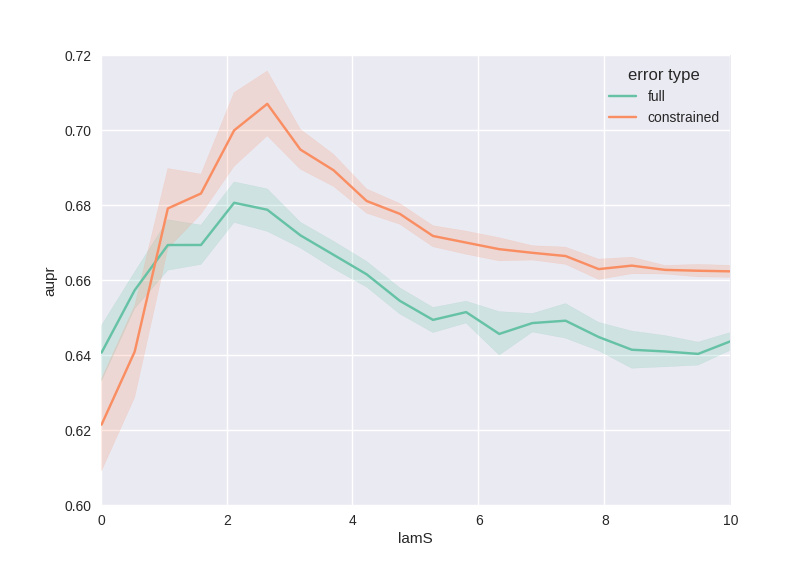
\includegraphics[scale=0.45]{simulated.png}
  \caption{\label{fig:figure1} This is what a figure looks like}
  \end{center}
\end{figure}

\section{Methods}
\subsection{GRN}
are good
\subsection{fused GRN}
yeees
\subsection{Simulated data}
Generation of simulated data begins with the production of random orthology mappings. We produce a one-to-one orthology by pairing random genes until a specified fraction have been assigned orthologs. This process is carried out seperately for TFs and non-TF genes, so that TFs and non-TF genes are never assigned to be orthologous. We then produce a pair of random networks ($B^1$ and $B^2$) as follows. For each unfilled entry in $B^1$ or $B^2$, we enumerate the set $C$ consisting of the entry along with every entry in either matrix to which it is fused. With probability equal to the sparsity rate we assign every entry in $C$ to be 0, otherwise we sample a value $v \sim \mathcal{N}(0,1)$ and independently assign each entry in $C$ to $v + \mathcal{N}(0, \sigma_f^2)$. $\sigma_f$ is a parameter that controls the distribution of differences in the values of fused coefficients, so that the nonzero coefficients of $B^1, B^2$ are distributed as $\mathcal{N}(0, 1 + \sigma_f^2)$.

Given a network $B$, we generate $N$ samples of gene expressions at each of two timepoints. The condition by gene expression matrix for timepoint one, $Y_{T1}$, is sampled randomly from a multivariate Gaussian distribution with identity covariance matrix. $X_{T1}$ is the TF expression sub-matrix of $Y_{T1}$, and consists of columns of $Y_{T1}$ that correspond to TFs. The gene expression matrix at timepoint two, $Y_{T2}$ is sampled as $Y_{T2} = Y_{T1} + BX_{T1}$. This process is carried out separately for each network. 

Following generation of simulated data, we may introduce error into the orthology mapping. This can take the form of discarding a specified fraction of true orthologies (governed by a false-negative rate), or by introducing random false orthologies (governed by a false-positive rate). For convenience, the false-positive rate is specified in units of the number of true orthologs, and not the number of possible orthologs. Priors are defined by the support of $B$. We can introduce false-positive or false-negative errors, as in the orthology mapping, in order to study the effect of faulty prior information. 
\subsection{Bacterial data}
is good
Look an equation array
\begin{equation}
\begin{array}{l}
R_i^{\mathrm{input}}(\theta) = c g_i^{\mathrm{input}}\exp(-(\theta - \theta_i)^2 / (2\sigma^2_{\mathrm{input}}))
\\
R_i^{\mathrm{output}}(\theta) = g_i^{\mathrm{output}}\sum_{j=0}^N R_j^{\mathrm{input}}(\theta) \exp(-(\theta_i - \theta_j)^2/(2\sigma^2_{\mathrm{output}})) .
\end{array}
\end{equation}
\bibliographystyle{plain}
\bibliography{paper}

\end{document}

